\subsection{Máquina de estados}\label{maquinaEdos}
Dentro del desarrollo de videojuegos existen personajes no jugables, abreviados como NPC del inglés (no playable character) y para su funcionamiento se utilizan diferentes métodos o teorías.
Dado que existia como riesgo acciones lineales o repetitivas para los jefes enemigos se decidió por emplear la teoría de autómatas.
Para las acciones del jefe en los niveles tres, cinco, siete y nueve se utiliza un autómata finito. El estado final es "Morir", donde este representa la destrucción del objeto. 
	\\[1pt]
	
\subsubsection{Jefe nivel 3}
Dada las acciones descritas anteriormente en el documento de diseño, se tiene coraza, impacto, lluvida de rocas, rugido. Además se agregan otras acciones no contempladas para la ayuda de transiciones.
La nomenclatura queda como sigue:
	\\[1pt]
	
\begin{itemize}
	\item Morir -> Mo
	\item Coraza -> Co
	\item Impacto -> Im
	\item Correr x4 -> Cx4
	\item Correr x1 -> Cx1
	\item Rugido -> RA
	\item Lluvia de rocas -> LR
	\item Vida 0 -> V0
	\item Esperar 2 seg. -> E2s
	\item Esperar 1 seg. -> E1s
	\item Jugador cerca -> Jc
\end{itemize}
	\\[1pt]

Los estados son:
	\\[1pt]
	Q = {Mo, Co, Im, Cx4, Cx1, RA, LR}
		\\[1pt]
		
El alfabeto son:
	\\[1pt]
	\sigma = {Jl, V0, E2s, E1s, Jc}
		\\[1pt]
		
El estado inicio es:
	\\[1pt]
	q0 = {LR}
		\\[1pt]
		
El estado final es:
	\\[1pt]
	F = {Mo}
		\\[1pt]

Como vemos en la imagen \ref{fig:maqN3} queda representada la máquina de estados.
\begin{figure}
	\centering
	\caption{Máquina de estados que realiza el jefe del nivel 3}
	\label{fig:maqN3}
	\includegraphics[width=0.5\textwidth]{imagenes\N3}
\end{figure}

\subsubsection{Jefe nivel 5}
Dada las acciones descritas anteriormente en el documento de diseño, se tiene ventisca y tornado. Además se agregan otras acciones no contempladas para la ayuda de transiciones.
La nomenclatura queda como sigue:
\\[1pt]

\begin{itemize}
	\item Morir -> Mo
	\item Estático x4 -> Ex4
	\item Estático x2 -> Ex2
	\item Tornado -> To
	\item Ventisca -> Ve
	\item Vida 0 -> V0
	\item Jugador lejos -> Jl
	\item Esperar 1 seg. -> E1s
	\item Jugador cerca -> Jc
\end{itemize}
\\[1pt]

Los estados son:
\\[1pt]
Q = {Mo, Ex4, Ex2, To, Ve}
\\[1pt]

El alfabeto son:
\\[1pt]
\sigma = {Jl, V0, E1s, Jc}
\\[1pt]

El estado inicio es:
\\[1pt]
q0 = {Ex4}
\\[1pt]

El estado final es:
\\[1pt]
F = {Mo}
\\[1pt]

Como vemos en la imagen \ref{fig:maqN5} queda representada la máquina de estados.

\begin{figure}
	\centering
	\caption{Máquina de estados que realiza el jefe del nivel 5}
	\label{fig:maqN5}
	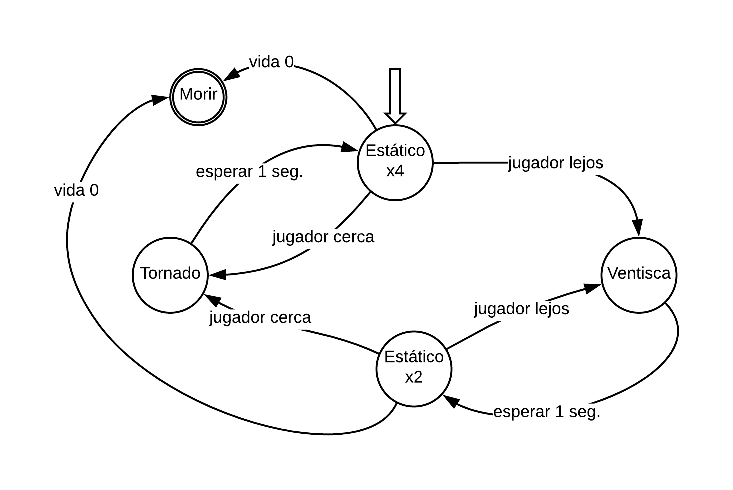
\includegraphics[width=0.5\textwidth]{imagenes\N5}
\end{figure}

\subsubsection{Jefe nivel 7}
Dada las acciones descritas anteriormente en el documento de diseño, se tiene lluvia de flechas, manotazo, lava. Además se agregan otras acciones no contempladas para la ayuda de transiciones.
La nomenclatura queda como sigue:
\\[1pt]

\begin{itemize}
	\item Morir -> Mo
	\item Estático x4 -> Ex4
	\item Estático x3 -> Ex3
	\item Estático x2 -> Ex2
	\item Manotazo -> Ma
	\item Lava -> La
	\item Lluvia flechas -> Lf
	\item Vida 0 -> V0
	\item Rand 0 -> R0
	\item Rand 1 -> R1
	\item Rand 2 -> R2
\end{itemize}
\\[1pt]

Los estados son:
\\[1pt]
Q = {Mo, Ex4, Ex2, Ex3, Ma, La, Lf}
\\[1pt]

El alfabeto son:
\\[1pt]
\sigma = {V0, R0, R1, R2}
\\[1pt]

El estado inicio es:
\\[1pt]
q0 = {Ex3}
\\[1pt]

El estado final es:
\\[1pt]
F = {Mo}
\\[1pt]


Como vemos en la imagen \ref{fig:maqN7} queda representada la máquina de estados.

\begin{figure}
	\centering
	\caption{Máquina de estados que realiza el jefe del nivel 7}
	\label{fig:maqN7}
	\includegraphics[width=0.5\textwidth]{imagenes\N7}
\end{figure}

\subsubsection{Jefe nivel 9}
Dada las acciones descritas anteriormente en el documento de diseño, se tiene estocada, filo y sablazo. Además se agregan otras acciones no contempladas para la ayuda de transiciones.
La nomenclatura queda como sigue:
\\[1pt]

\begin{itemize}
	\item Morir -> Mo
	\item Estocada -> Es
	\item Estático x4 -> Ex4 
	\item Sablazo -> Sa
	\item Filo -> Fi
	\item Jugador lejos -> Jl
	\item Rand 1 -> R1
	\item Rand 0 -> R0
	\item Vida 0 -> V0
	\item Esperar 1 seg. -> E1s
	\item Jugador cerca -> Jc
\end{itemize}
\\[1pt]

Los estados son:
\\[1pt]
Q = {Mo, Ex4, Es, Sa, Fi}
\\[1pt]

El alfabeto son:
\\[1pt]
\sigma = {Jl, Jc, E1s, R1, R0}
\\[1pt]

El estado inicio es:
\\[1pt]
q0 = {Ex4}
\\[1pt]

El estado final es:
\\[1pt]
F = {Mo}
\\[1pt]


Como vemos en la imagen \ref{fig:maqN9} queda representada la máquina de estados.
\begin{figure}
	\centering
	\caption{Máquina de estados que realiza el jefe del nivel 9}
	\label{fig:maqN9}
	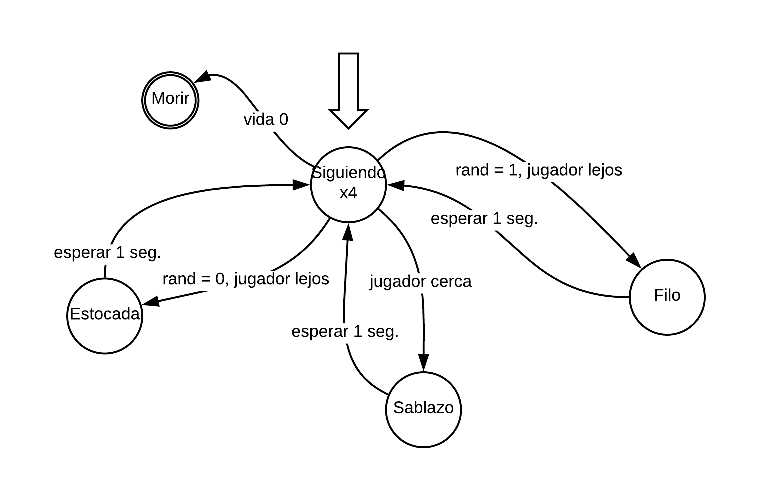
\includegraphics[width=0.5\textwidth]{imagenes\N9}
\end{figure}